\documentclass[11pt,a4paper]{article}

% ---------- Idioma y codificación (babel-spanish no está disponible: rótulos fijados a mano)
\usepackage[utf8]{inputenc}
\usepackage[T1]{fontenc}
\usepackage[english]{babel}
\renewcommand{\abstractname}{Resumen}
\renewcommand{\refname}{Referencias}
\renewcommand{\figurename}{Figura}
\renewcommand{\tablename}{Tabla}
\renewcommand{\contentsname}{Contenido}

% ---------- Paquetes
\usepackage[a4paper,margin=2.3cm]{geometry}
\usepackage{amsmath,amssymb}
\usepackage{graphicx}
\usepackage{booktabs}
\usepackage{caption}
\usepackage{float}
\usepackage[numbers,sort&compress]{natbib}
\usepackage{xcolor}
\usepackage{hyperref}
\graphicspath{{../figuras/}}
\captionsetup{font=small,labelfont=bf}

\title{\textbf{Análisis predictivo del circuito ATP:\\del ranking al historial de jugadores}}
\author{
  Juan Pablo Angonese, Agustín José Ceballos Pratto, Alan Yair Ghibaudo,\\
  Emanuel Genaro Scrosati, Genaro Villegas y Juan José Wendler\\[4pt]
  \small Universidad Tecnológica Nacional, Facultad Regional Córdoba, Argentina\\
  \small Trabajo práctico de Ciencia de Datos (curso 5K2, 2026), grupo N.\textordmasculine\,4
}
\date{}

\begin{document}
\maketitle

\begin{abstract}
Predecir el ganador de un partido de tenis profesional es un problema con datos abundantes y resultados difíciles de anticipar. Usamos 70.311 partidos del circuito ATP (2000--2026) para estimar la probabilidad de victoria de un jugador frente a otro, usando solo información disponible antes del partido. Las variables describen el historial de cada jugador: rating Elo general y por superficie, forma reciente, estadísticas de saque y devolución con medias móviles exponenciales, historial directo y ranking oficial. Evaluamos con un corte temporal (entrenamiento antes de 2024, test entre 2024 y 2026) y con predicción simétrica para eliminar el orden arbitrario de los jugadores. El ensamble de regresión logística, Random Forest y Gradient Boosting alcanza 64,6\,\% de accuracy y un ROC-AUC de 0,714 en test, frente a 63,7\,\% y 0,689 de la regla ``gana el mejor rankeado''. Un análisis de ablación muestra que el historial, sin ver el ranking, iguala al modelo completo, y el Elo es la familia de variables más influyente. Las probabilidades están bien calibradas: cuando el modelo asigna más de 90\,\% al favorito, este gana el 94\,\% de las veces. Presentamos además un simulador de torneos que explica la probabilidad de cada ronda. Discutimos los límites del enfoque, incluido el techo que impone el azar.
\end{abstract}

\noindent\textbf{Palabras clave:} predicción deportiva, tenis, Elo, validación temporal, calibración, aprendizaje automático.

\section{Introducción}

Un partido de tenis profesional enfrenta a dos jugadores con historias, superficies y momentos de forma muy distintos. Anticipar al ganador interesa a analistas, medios y equipos técnicos que preparan un rival. La práctica habitual es mirar el ranking oficial, que resume los puntos acumulados en las últimas 52 semanas. Esa simplificación tiene dos problemas: penaliza a jugadores que vuelven de una lesión o que compiten poco, y no distingue un rendimiento sostenido de uno reciente.

Este trabajo busca responder si el historial completo de cada jugador mejora la predicción del ganador, y cuánto. Nuestras contribuciones son:
\begin{itemize}
  \item Un proceso de limpieza y transformación documentado para una base pública de partidos ATP, con decisiones justificadas por la distribución de cada variable y por reglas del dominio.
  \item Un diseño de evaluación que evita la fuga de información: variables calculadas solo con partidos anteriores, corte temporal y predicción simétrica.
  \item Un conjunto de variables de historial (Elo general y por superficie, forma, saque, devolución, historial directo) con su comparación frente al ranking mediante ablación e importancia por permutación agrupada.
  \item Un análisis de calibración de las probabilidades, un caso de uso y un simulador de torneos.
\end{itemize}

\section{Trabajos relacionados}

El sistema Elo \cite{elo1978} estima el nivel de un jugador a partir de sus resultados y del nivel esperado de sus rivales, y se actualiza con cada partido. Es la base de las variables de nivel de nuestro trabajo. Kovalchik \cite{kovalchik2016} compara métodos de predicción de partidos de tenis, incluidos modelos basados en ranking y en estadísticas de partido.

Usamos tres familias de modelos: regresión logística regularizada, Random Forest \cite{breiman2001} y Gradient Boosting \cite{friedman2001}. Para la importancia de variables seguimos el enfoque de permutación de Breiman \cite{breiman2001}, agrupando variables correlacionadas. La validación respeta el orden temporal, como recomiendan Bergmeir y Benítez \cite{bergmeir2012}. Para evaluar la calidad de las probabilidades usamos Log-Loss, el puntaje de Brier \cite{brier1950} y la curva ROC \cite{fawcett2006}, y analizamos la calibración como se hace en \cite{guo2017}.

\section{Datos}

\subsection{Fuente y volumen}

Usamos la base TML-Database \cite{tml2026}, que recopila resultados del circuito ATP a partir de un scraping de la fuente oficial y de las bases abiertas de Sackmann \cite{sackmann}. La tabla de partidos contiene 78.091 registros entre 2000 y 2026, con 50 columnas: torneo, superficie, nivel, ronda, datos de ambos jugadores, marcador, duración y estadísticas de saque y devolución. La tabla de jugadores aporta fecha de nacimiento, altura y mano hábil. Unimos ambas tablas por el identificador del jugador y conservamos 2.733 jugadores con actividad en el período.

\subsection{Calidad de datos}

La Tabla~\ref{tab:calidad} resume el estado antes y después del tratamiento. No hay filas duplicadas exactas. Los valores nulos en partidos bajan de 378.735 a cero.

\begin{table}[H]
\centering
\caption{Calidad de datos antes y después del tratamiento.}
\label{tab:calidad}
\begin{tabular}{lrr}
\toprule
Métrica & Antes & Después \\
\midrule
Partidos (filas) & 78.091 & 70.311 \\
Filas duplicadas & 0 & 0 \\
Valores nulos en partidos & 378.735 & 0 \\
Columnas en partidos & 50 & 59 \\
Jugadores (filas) & 7.643 & 2.733 \\
Valores nulos en jugadores & 38.254 & 109 \\
\bottomrule
\end{tabular}
\end{table}

La falta de estadísticas no es uniforme. Copa Davis y Juegos Olímpicos tienen 80,1\,\% y 57,8\,\% de partidos sin datos de juego, y se disputan con un formato distinto al del circuito. Los excluimos (Figura~\ref{fig:nulos}). En el resto de los niveles, los nulos son menores al 1\,\%.

\begin{figure}[H]
\centering
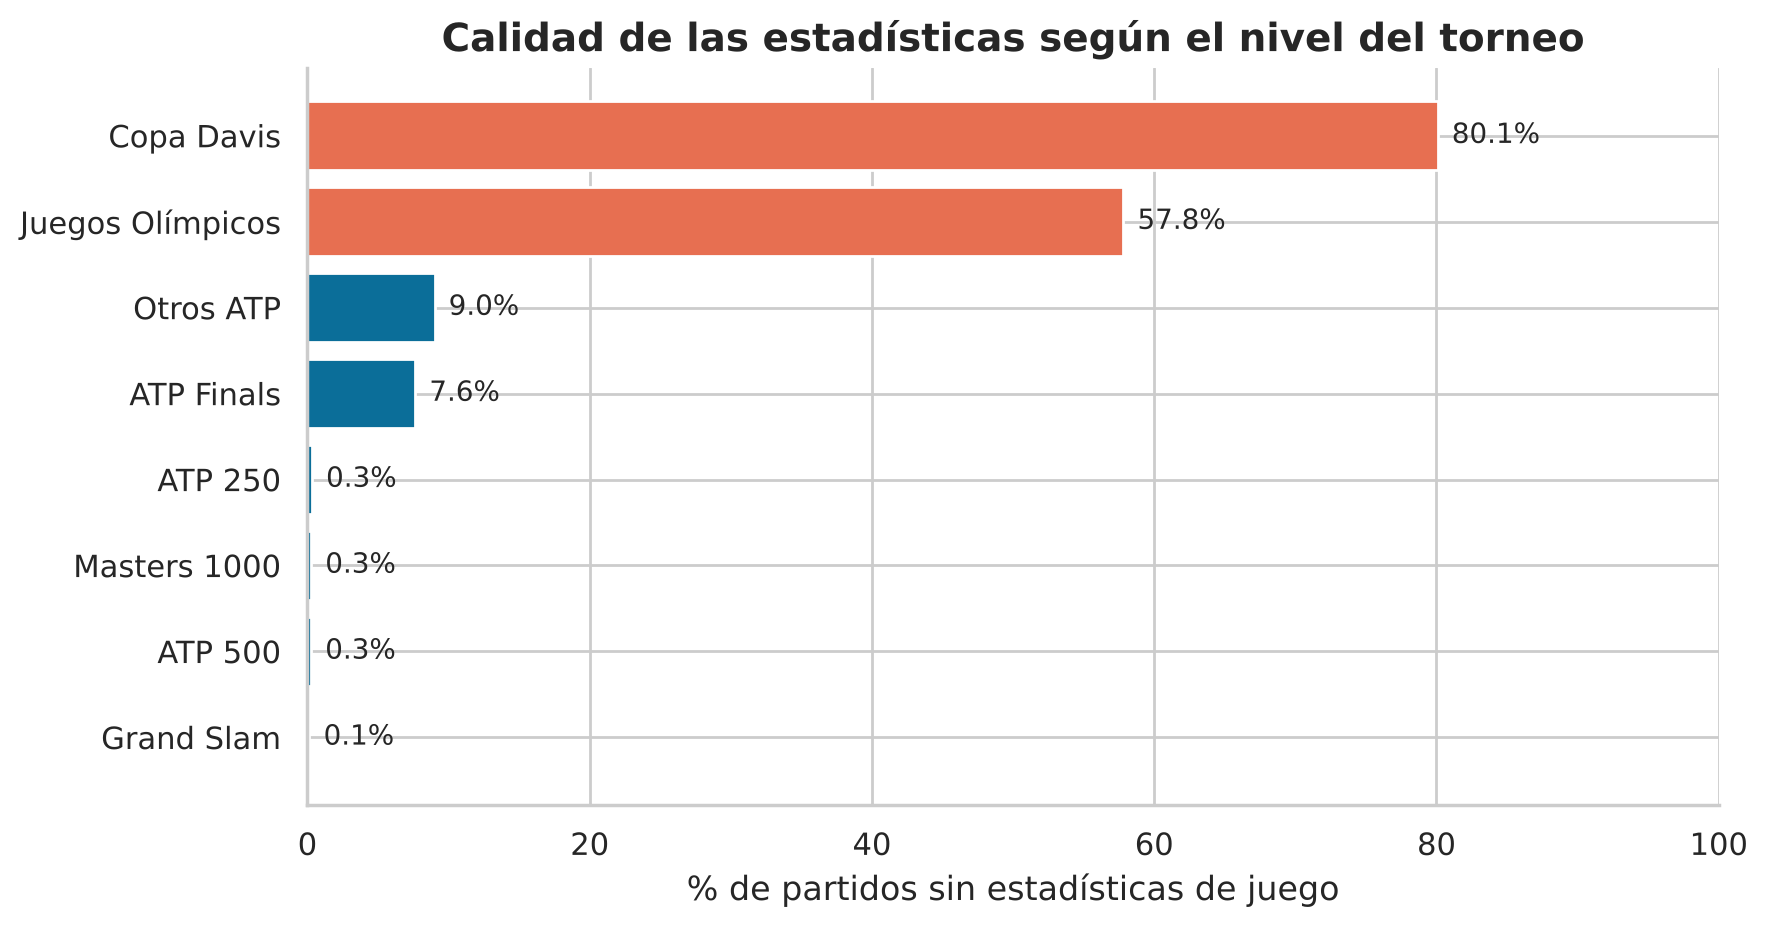
\includegraphics[width=0.8\linewidth]{fig02_nulos_por_nivel.png}
\caption{Porcentaje de partidos sin estadísticas de juego según el nivel del torneo. Los niveles en naranja se excluyen.}
\label{fig:nulos}
\end{figure}

Para los valores atípicos (outliers) en duración y altura no aplicamos eliminación masiva, porque un partido largo es un hecho real. Las imputaciones dependen de la distribución: la mediana para altura y edad, que son simétricas; la mediana por formato de sets para la duración, que tiene cola larga; y la mediana por superficie para las estadísticas faltantes. La Figura~\ref{fig:outliers} muestra la distribución antes y después.

\begin{figure}[H]
\centering
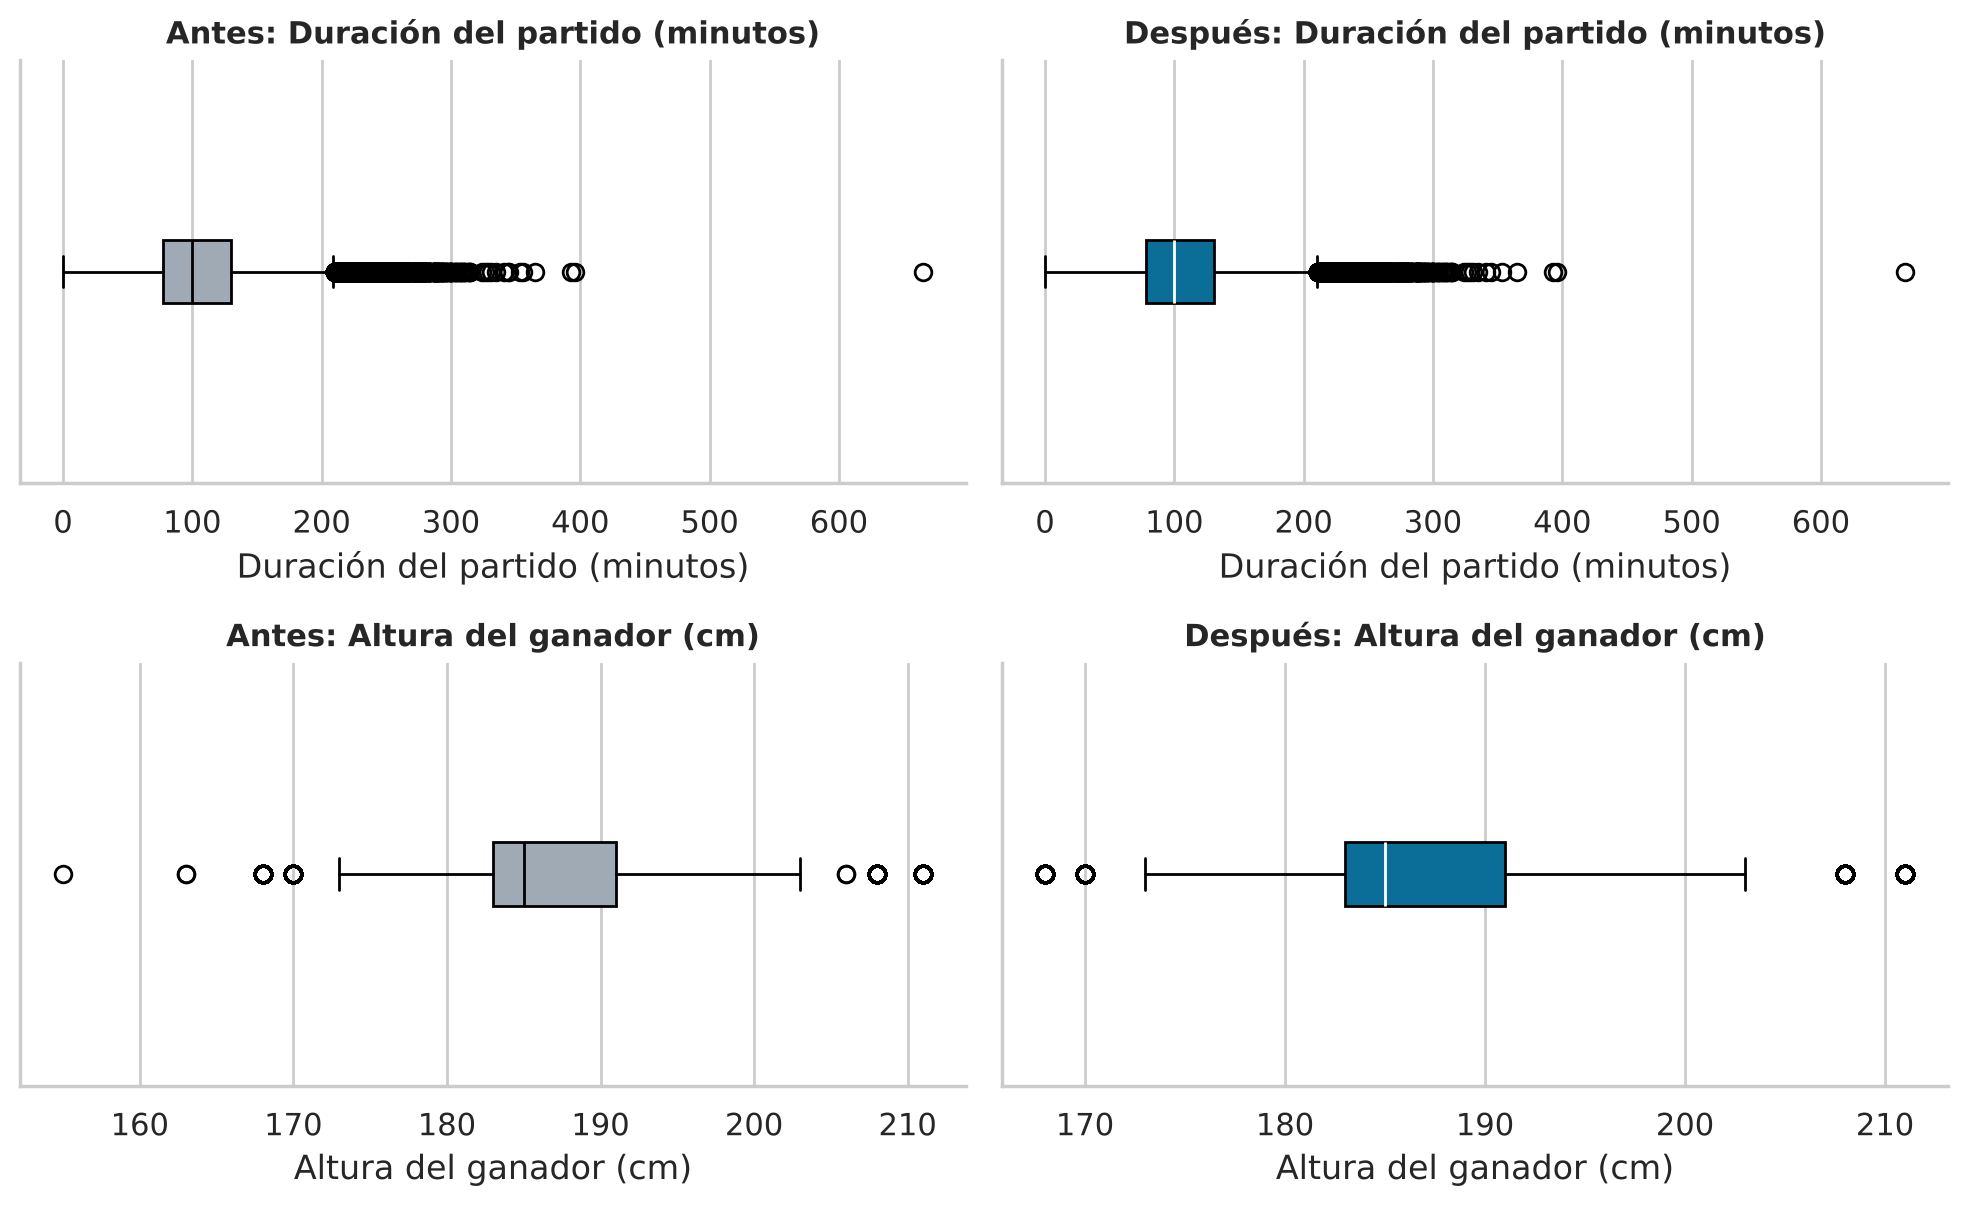
\includegraphics[width=0.85\linewidth]{fig11_pre_post_outliers.png}
\caption{Valores atípicos en duración del partido y altura del ganador, antes (izquierda) y después (derecha) del tratamiento.}
\label{fig:outliers}
\end{figure}

\section{Métodos}

\subsection{Variables}

Construimos 73 variables predictoras, agrupadas en ocho familias (Tabla~\ref{tab:familias}). Para cada jugador, calculamos sus variables con los partidos previos al partido que se predice; las estadísticas del propio partido nunca entran al modelo.

\begin{table}[H]
\centering
\caption{Familias de variables predictoras.}
\label{tab:familias}
\begin{tabular}{p{4.2cm}p{7.5cm}}
\toprule
Familia & Qué describe \\
\midrule
Ranking ATP & Posición y puntos oficiales \\
Elo general y por superficie & Nivel real, actualizado con cada resultado \\
Forma reciente & Victorias en los últimos 10 partidos \\
Superficie & Proporción de victorias en la superficie del partido \\
Saque & Efectividad de saque (media móvil exponencial) \\
Devolución & Puntos ganados al resto y break points convertidos \\
Historial directo & Victorias previas entre los dos jugadores \\
Físico y actividad & Edad, altura, experiencia y días sin competir \\
\bottomrule
\end{tabular}
\end{table}

Los conteos absolutos (aces, puntos de saque) dependen de la duración del partido, así que usamos porcentajes. Las estadísticas se promedian con una media móvil exponencial de ventana 20, para reflejar el nivel actual y no el de un período pasado.

\subsection{Rating Elo}

Cada jugador parte de 1.500 puntos. Tras cada partido, el ganador suma y el perdedor resta:
\begin{equation}
  E = \frac{1}{1 + 10^{(R_{\text{rival}} - R_{\text{jugador}})/400}}, \qquad R \leftarrow R + K\,(S - E),
\end{equation}
donde $S=1$ si gana y $S=0$ si pierde, y el factor de ajuste es $K = 250/(n+5)^{0{,}4}$, con $n$ la cantidad de partidos jugados. Así, un jugador nuevo se ajusta rápido y un veterano se estabiliza. Los walkovers no actualizan el rating. Calculamos un Elo general y otro por superficie.

\subsection{Orden cronológico y simetría}

Todos los partidos de un torneo comparten la fecha de inicio. Para evitar que una final aparezca antes que partidos previos, ordenamos por fecha, torneo, ronda y número de partido. Cada partido se representa de forma simétrica: asignamos al azar qué jugador es A (semilla fija). La predicción se hace en los dos sentidos (A contra B y B contra A) y se promedia, de modo que el resultado no depende del orden. Con esto, la clase positiva queda balanceada (50\,\%).

\subsection{Partición temporal y validación}

Entrenamos con 64.729 partidos anteriores al 1 de enero de 2024 (92,1\,\%) y evaluamos con 5.582 partidos entre esa fecha y el 17 de enero de 2026 (7,9\,\%). No usamos reparto aleatorio: con datos temporales permitiría entrenar con partidos posteriores a los que se predicen. La búsqueda de hiperparámetros usa validación cruzada temporal con cinco particiones, que siempre entrena con el pasado y valida con el período siguiente.

\subsection{Modelos e hiperparámetros}

Comparamos cuatro modelos con una línea base de dominio, la regla ``gana el mejor rankeado''. La Tabla~\ref{tab:modelos} muestra los hiperparámetros elegidos y el Log-Loss en validación cruzada. El criterio de selección fue el Log-Loss, porque el modelo entrega probabilidades y esta métrica penaliza las probabilidades exageradas.

\begin{table}[H]
\centering
\caption{Modelos candidatos, hiperparámetros elegidos y Log-Loss en validación cruzada temporal (menor es mejor).}
\label{tab:modelos}
\begin{tabular}{llp{4.6cm}r}
\toprule
Modelo & Idea central & Hiperparámetros elegidos & Log-Loss \\
\midrule
Regresión logística & Suma ponderada, pasada a probabilidad & $C=0{,}01$ (regularización L2) & 0,5907 \\
Random Forest & Árboles en paralelo, con votación & 150 árboles, profundidad 14, mínimo 20 partidos por hoja & 0,5935 \\
Gradient Boosting & Árboles en secuencia que corrigen errores & Tasa 0,03, profundidad 3, mínimo 100 partidos por hoja & 0,5916 \\
Ensamble (promedio) & Promedio de los tres anteriores & -- & \textbf{0,5901} \\
\bottomrule
\end{tabular}
\end{table}

El ensamble se eligió por ser el de menor Log-Loss en validación cruzada. La diferencia con la regresión logística es chica (0,0006), menor que el desvío entre particiones temporales (cerca de 0,0125). La ventaja del ensamble es real pero modesta.

\subsection{Métricas}

Usamos accuracy (proporción de aciertos), ROC-AUC, Log-Loss,
\begin{equation}
  \text{Log-Loss} = -\frac{1}{N}\sum_{i=1}^{N}\big[y_i\log p_i + (1-y_i)\log(1-p_i)\big],
\end{equation}
y el puntaje de Brier, $\frac{1}{N}\sum_i (p_i - y_i)^2$. Con el target simetrizado, la precisión, el recall y el F1 coinciden casi con el accuracy: un falso positivo y un falso negativo son el mismo error, es decir, elegir al jugador que perdió. Por eso no los usamos como criterio principal.

\section{Resultados}

\subsection{Desempeño en test}

La Tabla~\ref{tab:resultados} compara el modelo final con la línea base sobre los 5.582 partidos de test.

\begin{table}[H]
\centering
\caption{Desempeño en test (2024--2026).}
\label{tab:resultados}
\begin{tabular}{lrr}
\toprule
Métrica & Baseline (ranking) & Modelo final \\
\midrule
Accuracy & 63,7\,\% & \textbf{64,6\,\%} \\
ROC-AUC & 0,689 & \textbf{0,714} \\
Log-Loss & -- & \textbf{0,6166} \\
Brier & -- & \textbf{0,2148} \\
\bottomrule
\end{tabular}
\end{table}

La Figura~\ref{fig:comparacion} muestra la comparación entre modelos. Los cuatro modelos individuales están muy cerca entre sí, y todos superan al ranking. Esto sugiere que la información importa más que el algoritmo. La Figura~\ref{fig:confusion} muestra la matriz de confusión del modelo final. Por la simetrización, el eje ``gana A / gana B'' no tiene un significado especial: lo relevante es la diagonal.

\begin{figure}[H]
\centering
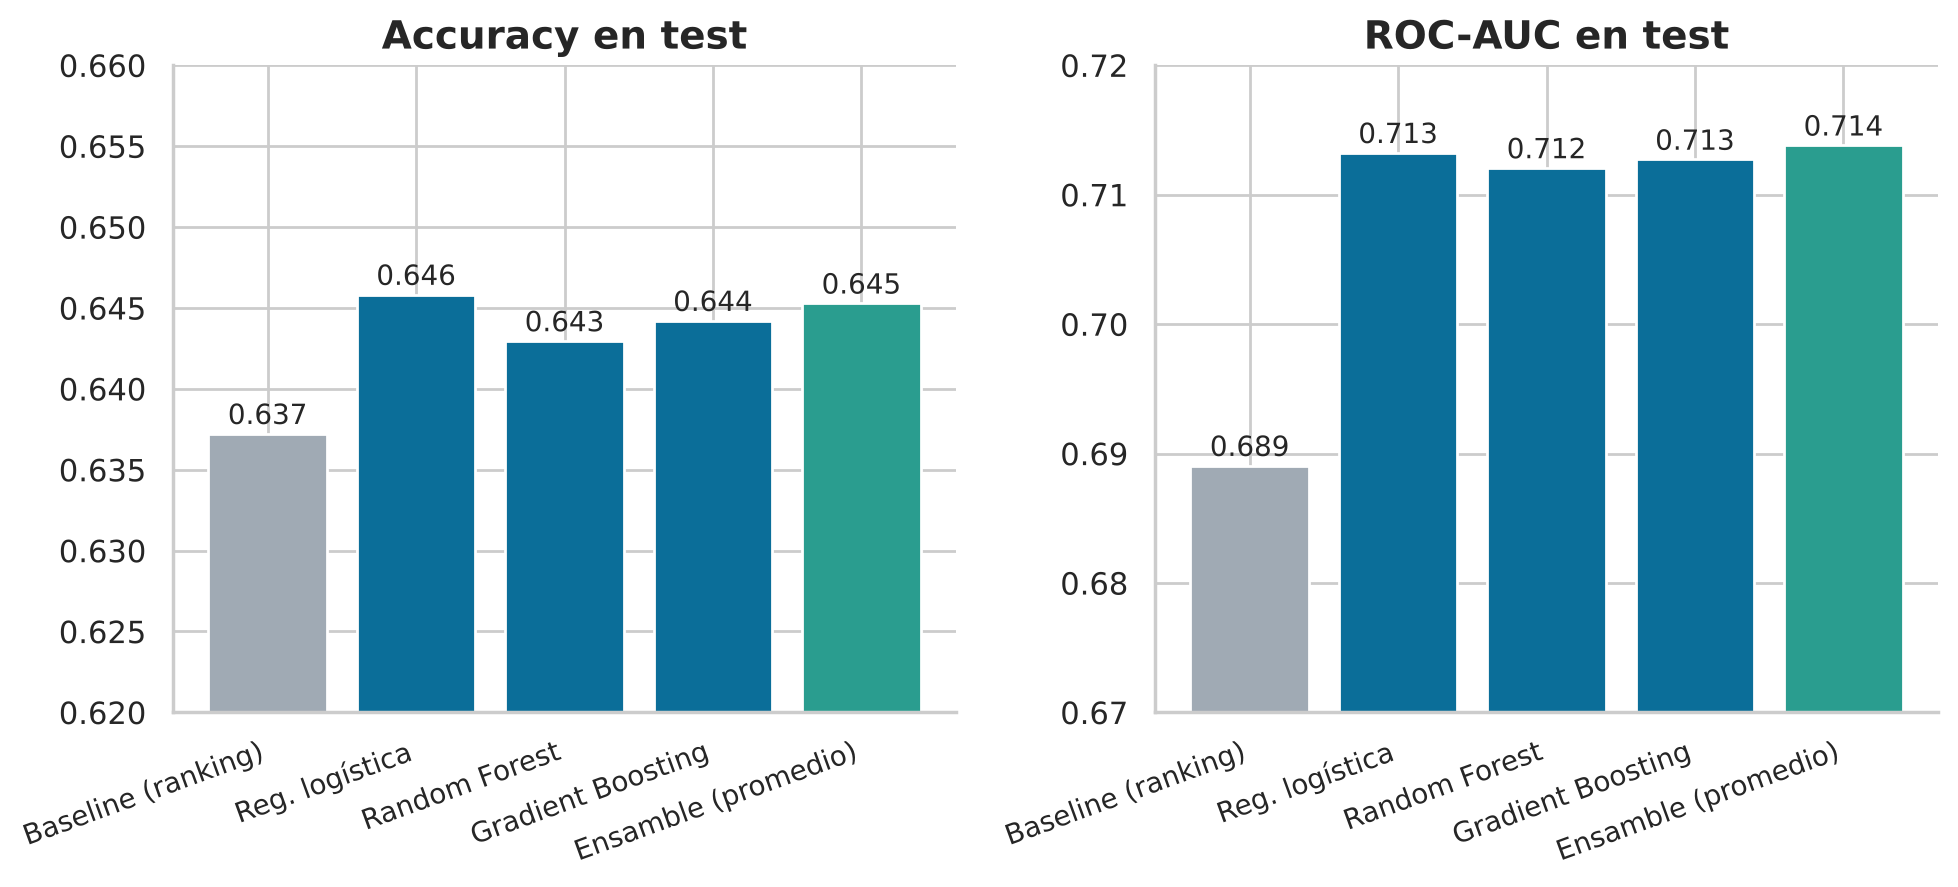
\includegraphics[width=0.85\linewidth]{fig04_comparacion_modelos.png}
\caption{Accuracy y ROC-AUC en test. Gris: baseline por ranking; azul: modelos individuales; verde: modelo final. Los ejes no parten desde cero.}
\label{fig:comparacion}
\end{figure}

\begin{figure}[H]
\centering
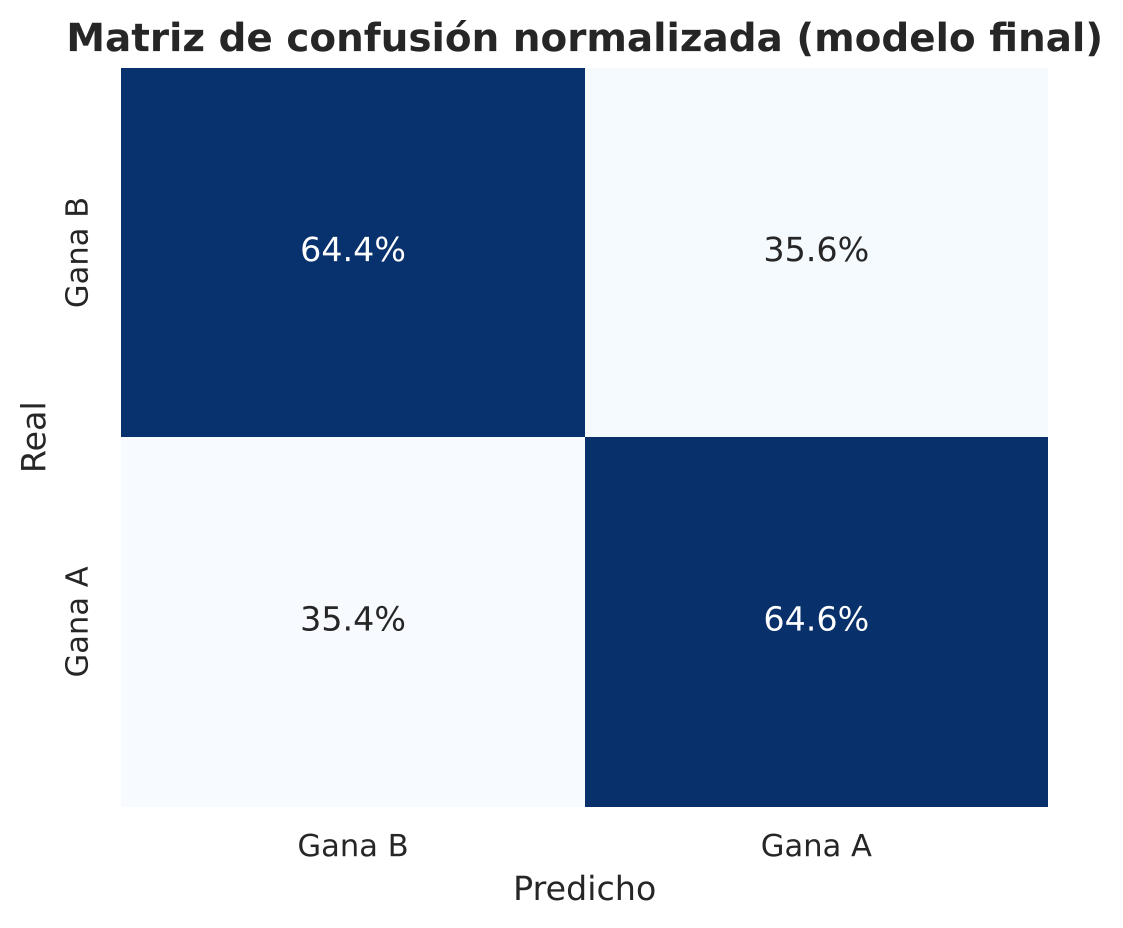
\includegraphics[width=0.55\linewidth]{fig10_matriz_confusion.png}
\caption{Matriz de confusión normalizada por fila del modelo final en test.}
\label{fig:confusion}
\end{figure}

\subsection{Calibración de las probabilidades}

Agrupamos los partidos de test según la confianza del modelo en el favorito (Figura~\ref{fig:calibracion}). En el tramo de 90 a 100\,\% (198 partidos), el modelo predijo 92,9\,\% y el favorito ganó 94,4\,\%. En los partidos entre jugadores del top 10 (120 partidos), el modelo asignó 67,1\,\% en promedio y el favorito ganó 70,8\,\%. En los tramos intermedios, la diferencia entre lo predicho y lo observado es de 2 a 3 puntos, con el modelo algo más optimista. En los favoritos muy claros, el modelo es algo más conservador. En conjunto, las probabilidades son razonablemente confiables, aunque no perfectas.

\begin{figure}[H]
\centering
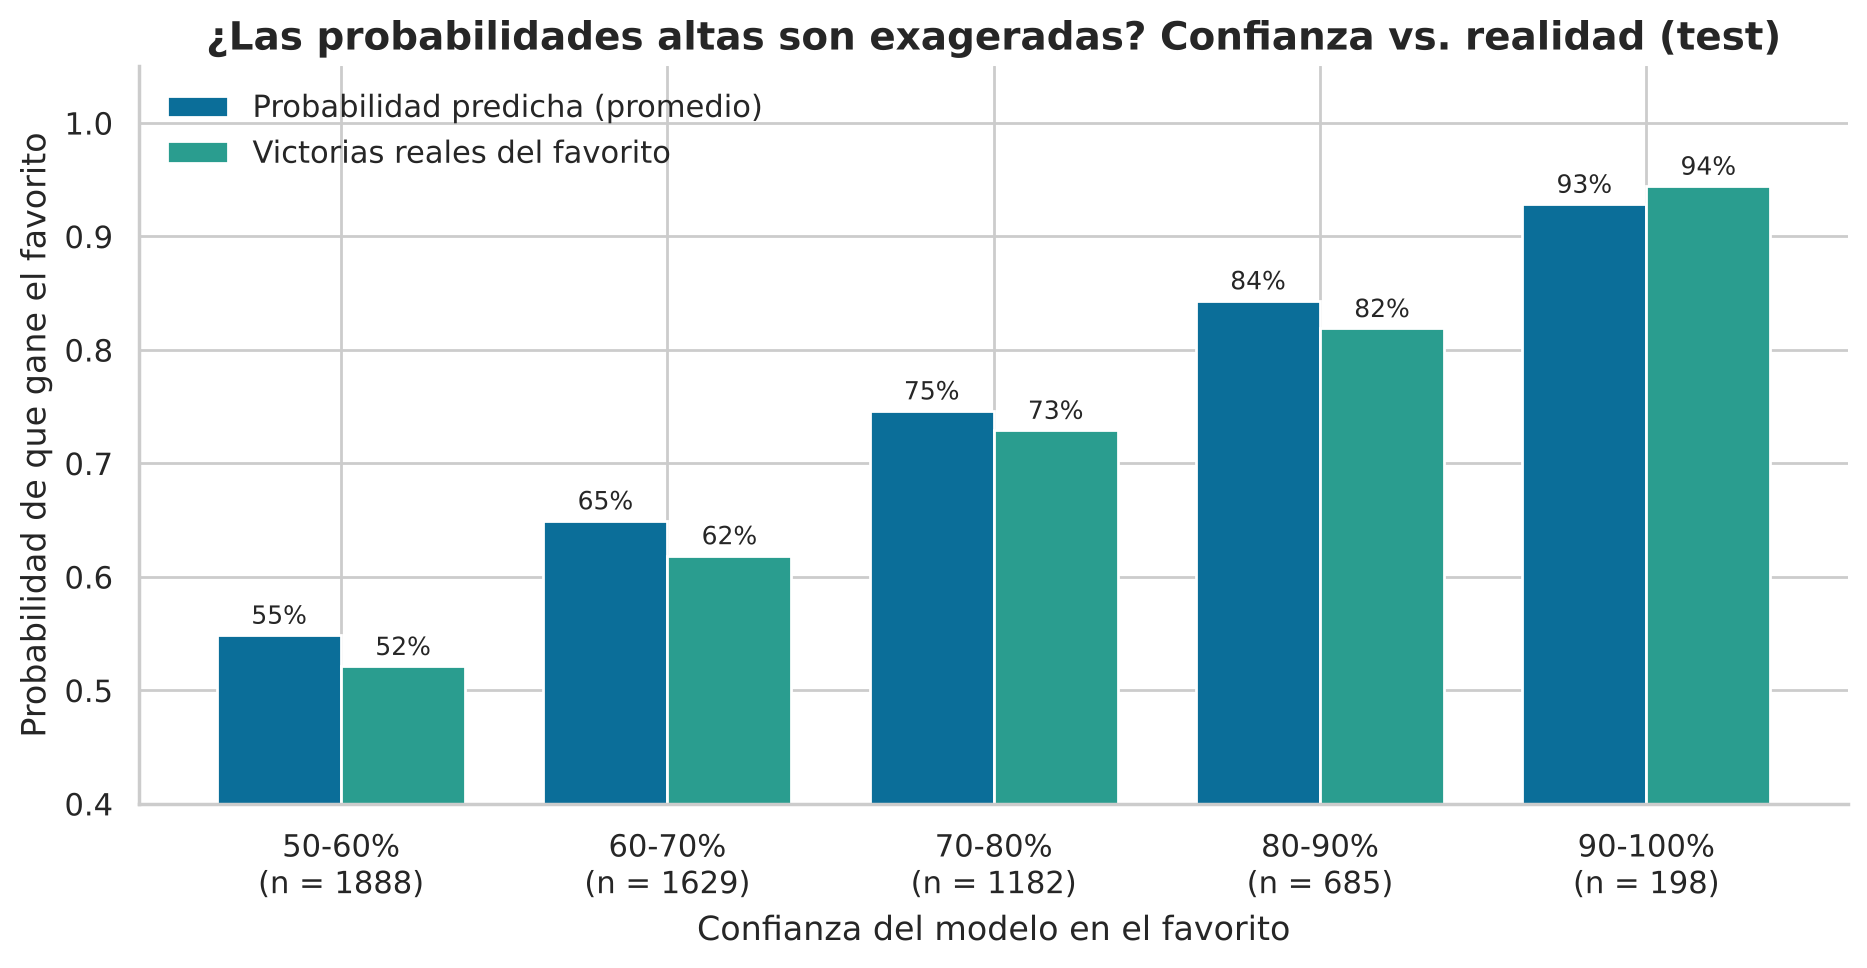
\includegraphics[width=0.8\linewidth]{fig06_calibracion_confianza.png}
\caption{Confianza del modelo en el favorito frente a la frecuencia real de victorias, en test. Si las barras tienen la misma altura, el modelo está bien calibrado.}
\label{fig:calibracion}
\end{figure}

\subsection{Ablación: ¿el modelo usa solo el ranking?}

Entrenamos tres versiones: solo ranking (9 variables), solo historial sin ranking (65 variables) y completo (73 variables). La Figura~\ref{fig:ablacion} muestra los resultados. El modelo sin ranking acierta 64,6\,\% (ROC-AUC 0,711), prácticamente igual que el completo (64,7\,\%; 0,713) y mejor que el ranking solo (63,3\,\%; 0,690). El historial contiene la información relevante, y el ranking es un resumen parcial de él.

\begin{figure}[H]
\centering
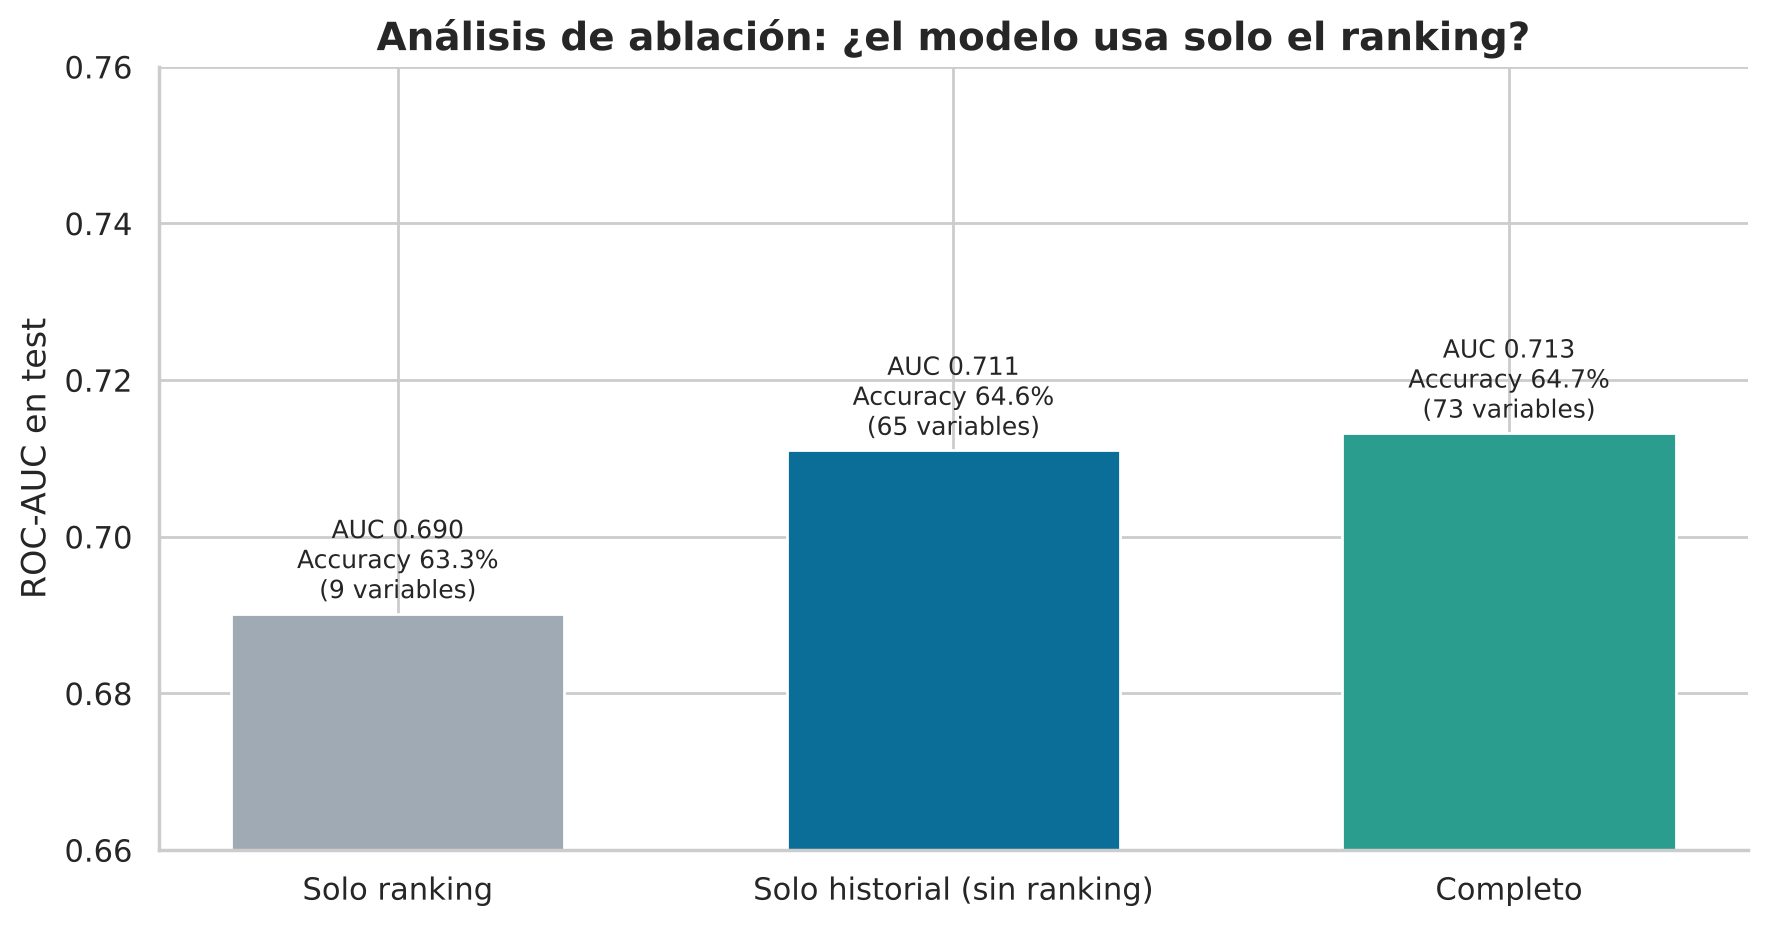
\includegraphics[width=0.8\linewidth]{fig07_ablacion.png}
\caption{ROC-AUC en test según el conjunto de variables utilizado.}
\label{fig:ablacion}
\end{figure}

\subsection{Importancia por familias de variables}

Medimos la importancia con permutación agrupada: desordenamos a la vez todas las variables de una familia y medimos la caída del ROC-AUC en test (promedio de cinco repeticiones sobre 4.000 partidos). Agrupar es necesario porque el Elo y los puntos de ranking están muy correlacionados: al desordenar una sola, la otra compensa y ambas parecen poco importantes.

El Elo general y por superficie cae 0,066, casi cuatro veces lo que cae el ranking (0,018). Le siguen el saque reciente (0,010) y el bloque físico y de actividad (0,007). La forma de los últimos 10 partidos (0,0001) y el historial directo (0,0006) aportan poco una vez que el modelo tiene medidas más finas de forma (Figura~\ref{fig:importancia}).

\begin{figure}[H]
\centering
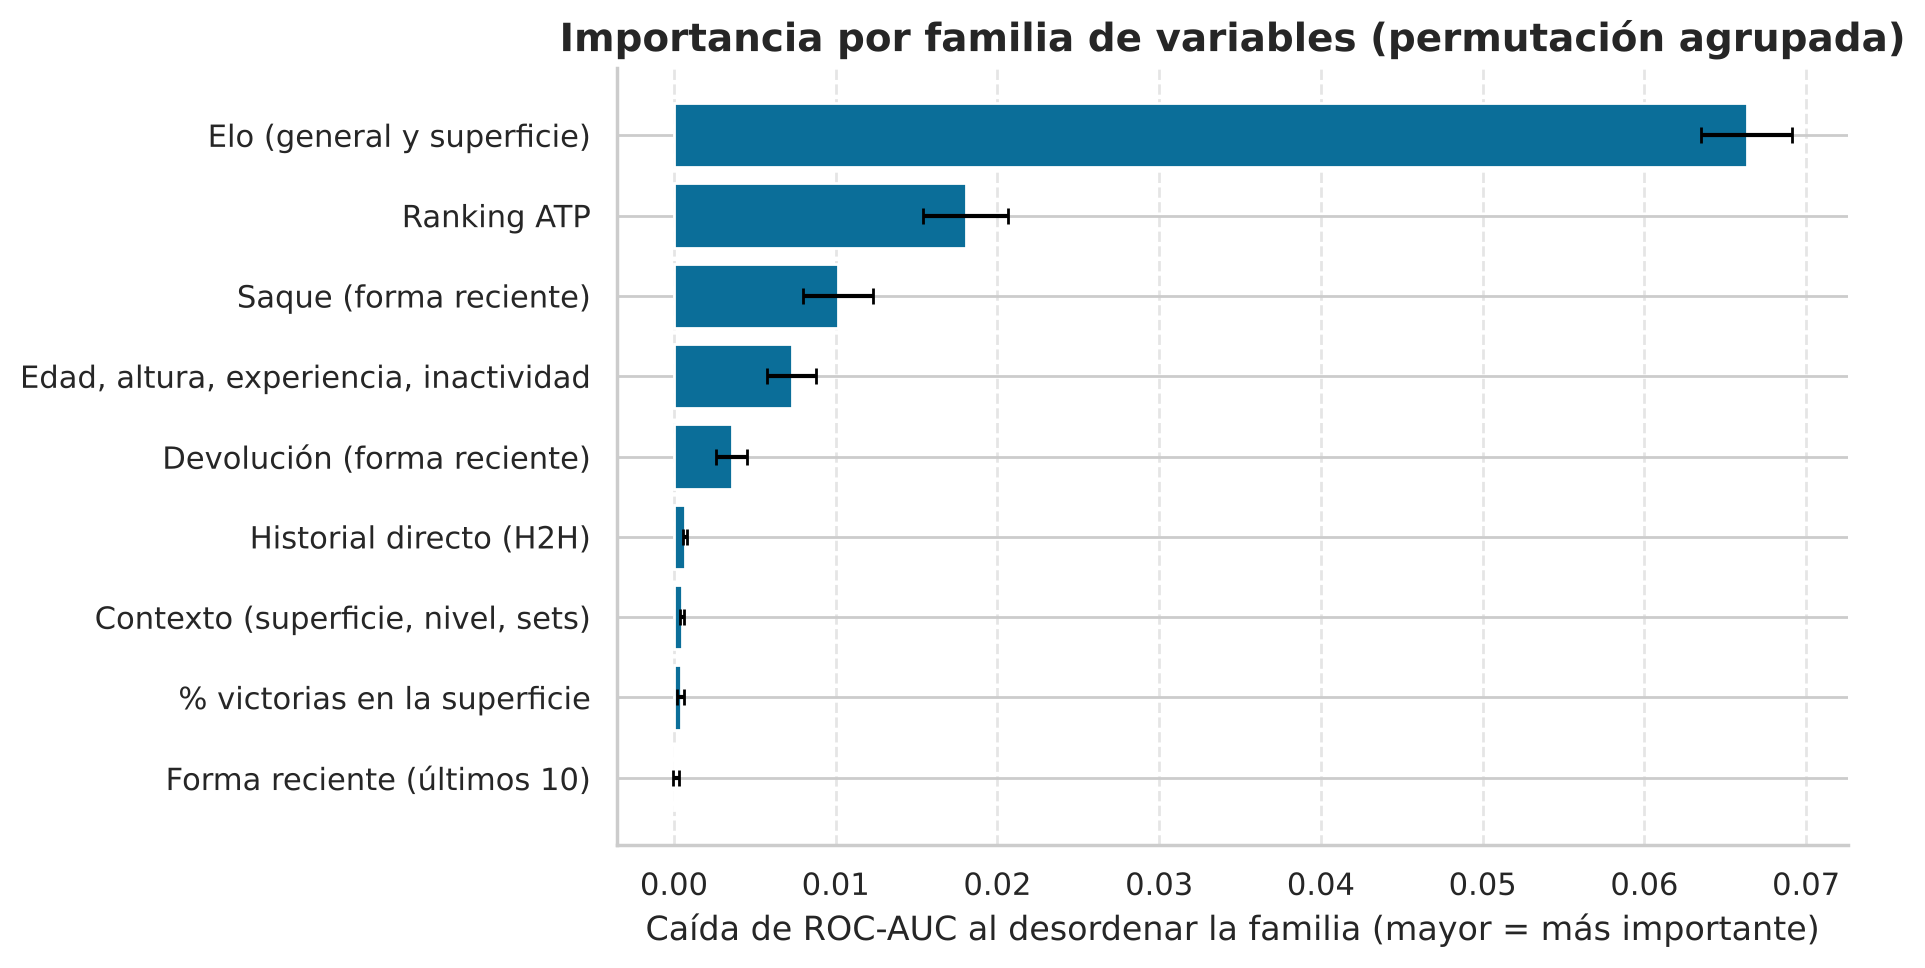
\includegraphics[width=0.8\linewidth]{fig08_importancia_familias.png}
\caption{Importancia por familia de variables: caída del ROC-AUC en test al desordenar la familia (barra negra: desvío).}
\label{fig:importancia}
\end{figure}

\subsection{Desempeño según el contexto}

La Figura~\ref{fig:contexto} compara el modelo con el ranking por superficie, nivel de torneo y diferencia de ranking. Los resultados son heterogéneos. En césped, el modelo mejora al ranking en 3,4 puntos (66,5\,\% frente a 63,1\,\%). En arcilla y cemento, la mejora es chica. En Grand Slam, el modelo acierta 72,7\,\% frente a 70,2\,\%. En Masters 1000, el ranking es mejor (63,8\,\% del modelo frente a 64,9\,\%). Cuando la diferencia de ranking supera los 250 puestos, el ranking acierta más (67,7\,\% frente a 66,1\,\%). Los niveles con muestras chicas, como ATP Finals (30 partidos), no se interpretan.

\begin{figure}[H]
\centering
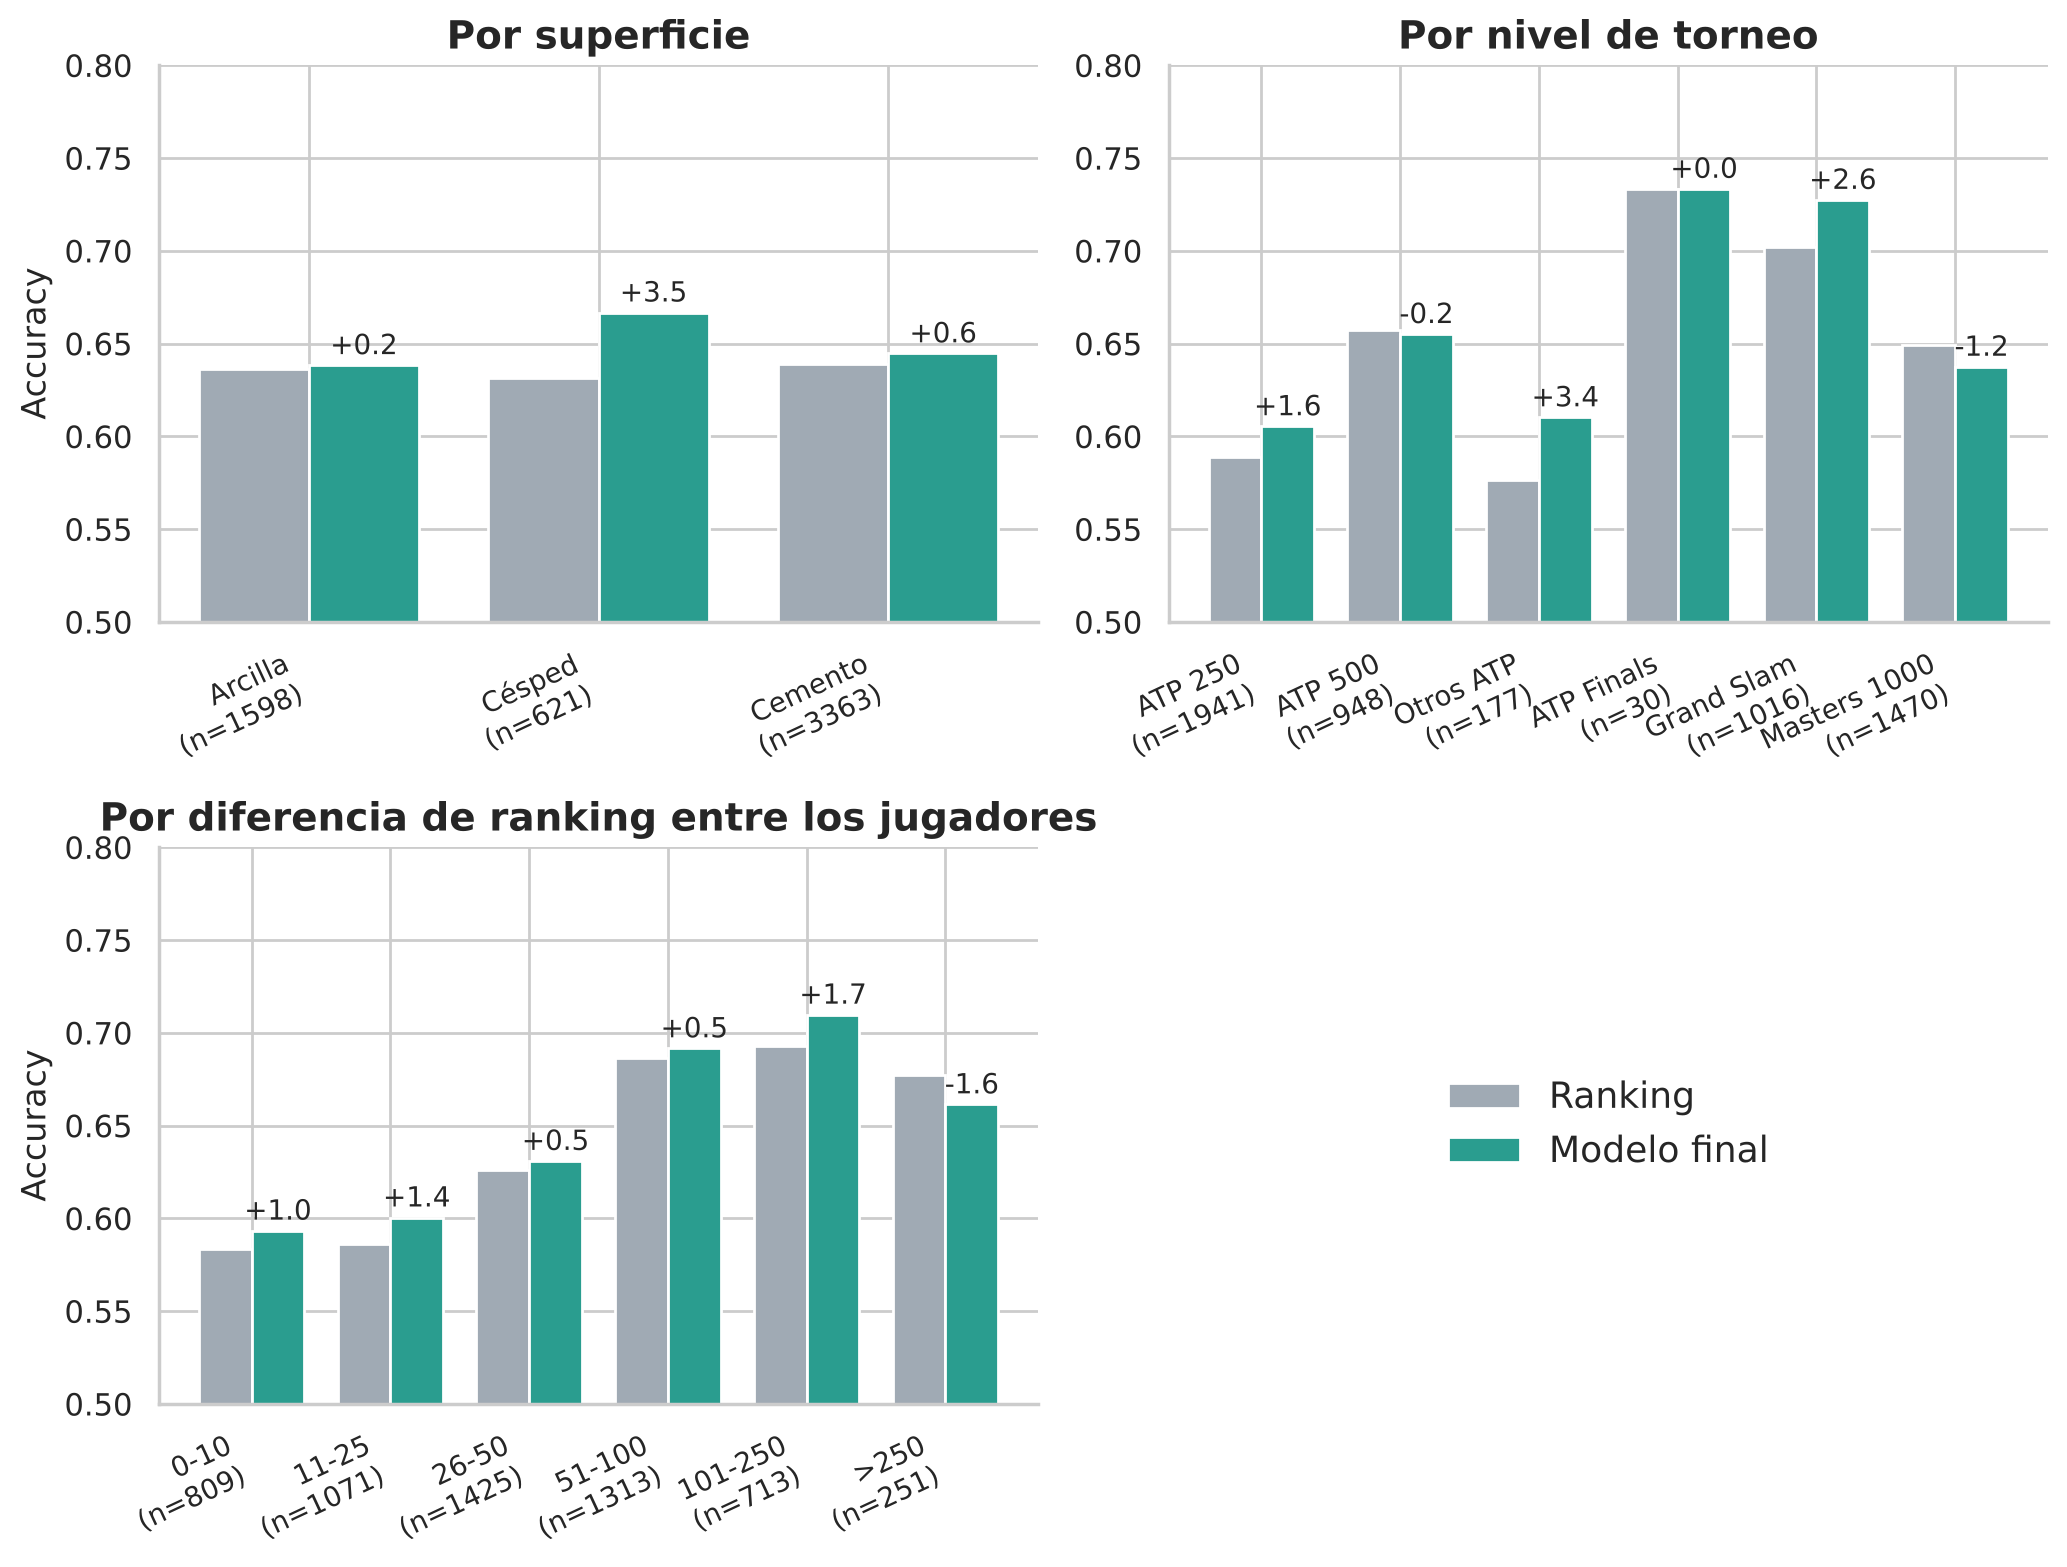
\includegraphics[width=0.95\linewidth]{fig09_accuracy_por_contexto.png}
\caption{Accuracy del ranking (gris) y del modelo final (verde) por superficie, nivel de torneo y diferencia de ranking. Los números indican la diferencia en puntos porcentuales.}
\label{fig:contexto}
\end{figure}

\subsection{Caso de uso}

Como ejemplo, consideramos un partido sobre arcilla entre Holger Rune (ranking 11, Elo sobre arcilla 1.917) y Valentin Vacherot (ranking 32, Elo sobre arcilla 1.448). El modelo asigna 75,5\,\% a Rune. La explicación por familias atribuye la mayor parte de esa diferencia al Elo general y por superficie (+15,7 puntos), seguido por la devolución reciente (+3,0) y el ranking (+2,9). Este caso ilustra cómo el modelo llega a su número; no valida el modelo por sí solo. Además, simulamos torneos de ocho jugadores y de 32 jugadores activos elegidos al azar, con la probabilidad de cada ronda y las variables que la explican.

\section{Discusión}

\textbf{Qué funcionó.} La combinación de Elo por superficie, saque y devolución con medias móviles exponenciales captura mejor el nivel actual de un jugador que el ranking oficial. La validación temporal y la predicción simétrica dieron una evaluación honesta: los resultados no dependen del orden arbitrario de los jugadores ni de datos posteriores al partido.

\textbf{Qué no funcionó del todo.} El algoritmo tiene poco efecto frente a la información: los cuatro modelos quedan muy cerca. La ventaja sobre el ranking es moderada (0,9 puntos de accuracy y 0,025 de ROC-AUC). En contextos con diferencias de ranking muy grandes, el ranking ya es suficiente.

\textbf{Límites.} El azar impone un techo: en torno al 36\,\% de los partidos del test los gana el peor rankeado. El modelo no incorpora lesiones, cansancio, clima ni cuotas de mercado. Las diferencias por contexto no tienen todavía pruebas de significancia estadística, y los niveles con pocas muestras deben leerse con cautela.

\section{Aspectos a mejorar}

Estas líneas quedan fuera de los resultados presentados. Son propuestas para una próxima iteración.

\begin{itemize}
  \item \textbf{Alternativas de reentrenamiento.} No evaluamos ponderar los partidos recientes ni limitar el histórico a partir de 2010. Ambas opciones podrían mejorar la estimación de la forma actual de los jugadores.
  \item \textbf{Cuotas de mercado.} Las cuotas resumen información pública previa al partido. Incorporarlas es una propuesta, sin cifras propias en este trabajo.
  \item \textbf{Lesiones y cansancio.} Son factores relevantes que hoy no están en la base de datos.
  \item \textbf{Evolución del rendimiento.} La trayectoria de cada jugador a lo largo de su carrera, planteada en la etapa de planificación, queda pendiente.
  \item \textbf{Significancia estadística.} Las diferencias por contexto, como la de Grand Slam, deberían evaluarse con un test sobre los mismos partidos (por ejemplo, McNemar).
  \item \textbf{Simulación de torneos.} Estimar la probabilidad de campeón requiere simular miles de cuadros, no un único escenario. Además, el cuadro de 32 jugadores usa formato de tres sets para un Grand Slam; conviene unificar el formato.
\end{itemize}

\section{Conclusiones}

Predecir el ganador de un partido de tenis profesional usando solo información previa al partido es posible con una mejora moderada sobre el ranking. El historial del jugador, en particular el Elo por superficie, aporta la información relevante. Las probabilidades del modelo son razonablemente confiables, sobre todo en los favoritos claros. El límite del azar es el principal obstáculo, y cualquier predicción previa al partido lo enfrenta. No recomendamos usar el modelo para apostar: la ventaja sobre el ranking es chica y no fue validada contra cuotas reales.

\section*{Disponibilidad de código y datos}

El código y el notebook con las salidas están en \url{https://github.com/genavillegas/atp-match-prediction}, bajo licencia MIT. El archivo \texttt{requirements.txt} fija las versiones de las librerías con las que reproducimos el notebook (scikit-learn 1.6.1, pandas 2.2.2, numpy 2.0.2). Con esas versiones, la regresión logística y el Random Forest coinciden con los valores reportados; Gradient Boosting difiere en pocas predicciones cercanas al umbral, por lo que el accuracy del ensamble puede dar 64,5\,\% en lugar de 64,6\,\%. Los datos provienen de TML-Database \cite{tml2026} y no se incluyen en el repositorio; deben consultarse con su licencia original.

\bibliographystyle{plainnat}
\bibliography{refs}

\end{document}
